\section{Client-server view (UML Component diagram)}\label{sec:client-server}

\begin{figure}[!htp]
    \centering
    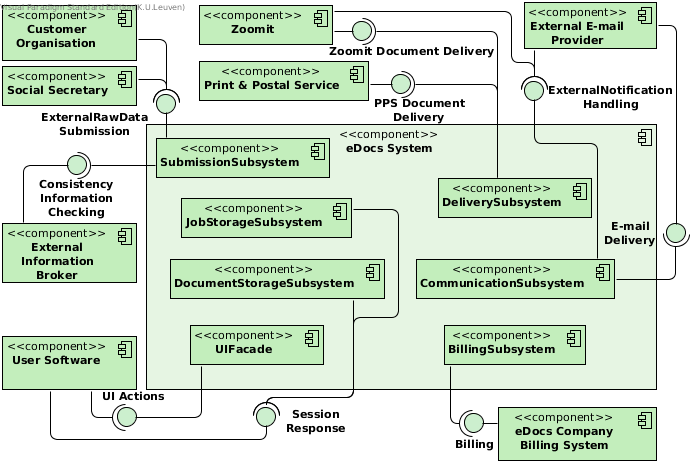
\includegraphics[width=0.8\textwidth]{figures/Context Diagram 1.png}
    %\missingfigure[figwidth=0.8\textwidth]{Context diagram of the client-server view.}
    \caption{Context diagram for the client-server view.}\label{fig:cc-context}
\end{figure}

In Figure \ref{fig:cc-context}, we present a context diagram of the client-server view, detailing the external communication to and from the system. The entry points to the system are the (mostly automated) external version of raw data submission. The Customer Organisation and/or Social Secretary can submit Raw Data Batches via the specified protocols supported by the eDocs system.
The other entry point being the \ttt{UIfacade}, which is contacted by User Software for User Interface Actions, e.g. a management dashboard for the Customer Administrator (one or more per Organisation) to query for job statuses, or a log-in system for recipients to log in to the PDS.
The exit points of the system are more versatile. There is one closely related to the UI Actions, where parts of the system respond to queries by directly supplying information to the user sessions, which in turn are individual (dedicated) intermediaries for instances of the client software. This bypasses the \ttt{UIFacade} as a bottleneck.
The \ttt{SubmissionSubsystem} queries an \ttt{External Information Broker} when verifying the meta-data of Raw Data Batches and Entries as specified in \emph{UC3}.
The \ttt{BillingSubsystem} contacts the \ttt{Billing System} (external of the actual eDocs system) used by the eDocs Company periodically to bill users of eDocs.
The \ttt{CommunicationSubsystem} submits composed e-mails to an \ttt{External Email Provider} for delivery. This functionality is used for reporting errors in the system to the eDocs admin, various notifications to CO admins, delivery of documents etc.
There are two other external communication mechanisms for document delivery, namely the \ttt{Zoomit} service's \ttt{Document Delivery} interface and the \ttt{Print \& Postal Service}'s one. These are both directly used by the delivery subsystem, in contrast to document delivery by e-mail, which passes through the \ttt{CommunicationSubsystem}, as explained earlier.

\begin{figure}[!htp]
    \centering
    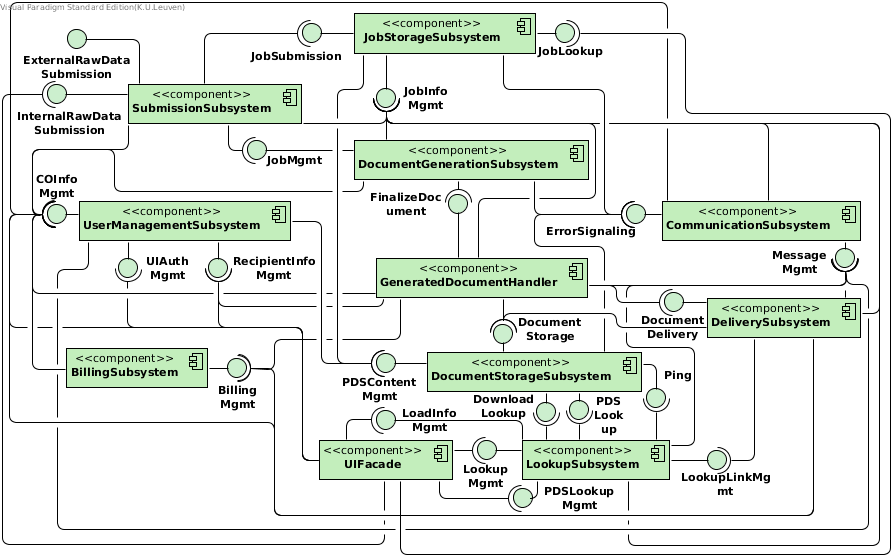
\includegraphics[width=\textwidth]{figures/Subsystem Diagram.png}
    %\missingfigure[figwidth=0.8\textwidth]{Primary diagram of the client-server view.}
    \caption{Primary component-and-connector view of the proposed architecture.}\label{fig:cs-primary}
\end{figure}

Figure \ref{fig:cs-primary} shows the primary component-and-connector diagram of the system. The presented overview divides the eDocs system into several subsystems, each with their dedicated functionalitie(s). The division are straightforward, and make for a less coupled system.\\
The \ttt{SubmissionSubsystem} accepts \ttt{Raw data batches} from an external user or via the \ttt{UIFacade}. It verifies these \ttt{Batches} and then registers them for generation in the \ttt{JobStorageSubsystem} and the \ttt{DocumentGenerationSubsystem}.\\
The \ttt{JobStorageSubsystem} stores the statuses of document generation and delivery jobs. It records raw data for document generation until said document has been succesfully generated succesfully. The \ttt{Subsystem} can be queried for job statuses, e.g. by the administrator of a Customer Organisation. It is contacted by the different subsystems concerned with the lifecycle of a document in the system, to record and update the document's status e.g. Waiting for generation, generated, delivered etc.\\
The \ttt{DocumentGenerationSubsystem} generates documents from submitted batches and applies scheduling based on deadlines of jobs. This generation consists of fetching the template for the document type of the document currently being generated, filling out the fields and any special steps befitting the document type (e.g. signing invoices). When finished, it hands the document to the \ttt{GeneratedDocumentHandler} for storage and delivery.\\
The \ttt{GeneratedDocumentHandler} is a passthrough point for generated documents. This component is not an actual subsystem, but an important branching point in the internal document flow. The \ttt{GeneratedDocumentHandler} determines for a document exactly where it has to go (e.g. whether e-mail actually means e-mail or should go to the PDS), and submits the document with the specific addressing data to both the \ttt{DeliverySubsystem} and the \ttt{DocumentStorageSubsystem}. It also marks a document as generated in the \ttt{JobStorageSubsystem}.\\
The \ttt{DocumentStorageSubsystem} is dedicated to the storage of documents. It has a database for \ttt{Personal Document Store} documents and a database for all documents; this means that the set of documents stored in the former is a subset of the set of documents stored in the latter. It also has an intermediary that makes constructing the \ttt{Personal Document Store} for newly registered Recipients more convenient on the one hand and an intermediary that contains a cache for documents to be stored in the \ttt{Personal Document Store} in case that database fails on the other.\\
The \ttt{DeliverySubsystem} performs the actual document delivery (or notification of a new document) to recipients. It manages all \ttt{Delivery Channels} and determines from the addressing data by the \ttt{GeneratedDocumentHandler} which \ttt{Channel} to use for delivery. It directly addresses the used external service for delivery (e.g. Zoomit, Print \& Postal Service), except in the case of email delivery. Composed delivery or notification e-mails are passed to and delivered by the \ttt{CommunicationSubsystem}.\\
The \ttt{CommunicationSubsystem} handles outbound communication. There is a channel for notifications due to internal systems failure and a channel for all other communication. Due to the requirement that eDocs administrators be notified of any kind of failure within one minute (see \emph{Av1} and \emph{Av2}), the error channel can temporarily suppress the other communication to ensure that error notifications get to their destination on time.\\
The \ttt{UserManagementSubsystem} stores all information regarding the different types of users and registered (non-authenticable) entities , which currently are: Recipients, Customer Administrators, actual Customer Organisations and eDocs Administrators. For the authenticable users, the \ttt{UserManagementSubsystem} provides authentication and authorization functionality, in turn supported by session logic in the \ttt{UIFacade}. The \ttt{Subsystem} provides functionality for the system to query info about Recipients, Customer organisations etc. and add or update this information (mostly by the eDocs administrator). Since the \ttt{UserManagementSubsystem} also governs whether a recipient is \emph{Registered} or not, the \ttt{Subsystem} notifies the \ttt{DocumentStorageSubsystem} to add or remove a recipient's documents in the PDS system.\\
The \ttt{BillingSubsystem} makes it possible to log any transaction consisting of document generation bills and document delivery bills, such that an invoice can be automatically sent to Customer Organizations for all activities performed on their behalf in a certain period. That period can be each month, each week or any other period length, whichever the financial department of eDocs deems most appropriate.\\
The \ttt{LookupSubsystem} processes requests for document lookups. It can handle requests where either a download link, a \ttt{JobID} or a search query is provided. In order to handle download links, there is a \ttt{LookupLinkCodec}, which can encode and decode downloads links (and also links specified to the \ttt{Personal Document Store}) and a \ttt{DownloadLinkCatalogue} where download links are stored for 30 days. If a Registered Recipient issues a query for the \ttt{Personal Document Store}, the \ttt{PDSLookupModule} handles that. To enable to system to throttle lookup requests (see \emph{P2}), there is a \ttt{LoadBalancer} which has to explicitly approve each lookup before it can be executed.\\
The \ttt{UIFacade} acts as an intermediary between all different kinds of user interfaces (a management dashboard, a Recipient PDS client etc.) and the system. The \ttt{UIFacade} passes all calls to the actual subsystems. It has a session infrastructure for user interface clients, so it is not one single bottleneck for all requests. The current different functionalities handled by the \ttt{UIFacade} are loging users in and out, registering new users, looking up job statuses and documents, submitting raw data through a dashboard and entering system information for load balancing in lookups.\\
Most of the previously named subsystems and components are further decomposed in Section \ref{sec:decomposition} to the required level of detail.

\subsection{Main architectural decisions}
In the following subsections we will discuss how the non-functional requirements are met by our architecture. The solutions and possible alternatives to the non-functional requirements are explained in the most self-contained way possible. Where necessary, references are made to Figure \ref{fig:cs-primary} and one or more decompostion views in section \ref{sec:decomposition}.

\subsubsection{Av1a and Av2a: notification of the eDocs Administrator}\label{march:av1a-av2a}
The \ttt{CommunicationSubsystem} provides notification functionality for all users. Since signaling an internal error of the system has precedence over most if not all other message traffic, the \ttt{CommunicationSubsystem} is split into an \ttt{ErrorEmailDeliveryHandler} and \ttt{NotificationEmailDeliveryHandler}. The former delivers notices about errors internal to the system, the latter all other notices. As stated before, for precedence of these error notifications, the \ttt{ErrorEmailDeliveryHandler} can throttle or temporarily halt any e-mail traffic from the \ttt{NotificationEmailDeliveryHandler}. This allows the system to alert the eDocs administrator(s) in a timely fashion, uner one minute, as stated in both \emph{Availability scenarios}.

\subsubsection*{Alternatives considered}
\paragraph{Alternative(s) for splitting the \ttt{EmailDeliveryHandler}s} All notifications could be submitted to one single \ttt{EmailDeliveryHandler}, together with a priority number. This allows said \ttt{EmailDeliveryHandler} to give precedence to certain notification, e.g. the internal error notification, but this could slow down the \ttt{CommunicationSubsystem} due to constant priority sorting, and can even lead to regular notification starvation (without the intervention of error notifications) in the most extreme of cases.

\subsubsection{Av1b: storing the status of an individual job}\label{march:av1b}
The \ttt{JobStorageSubsystem} is responsible for storing the status of individual jobs. For this purpose, a dedicated \ttt{JobStatusDatabase} is introduced to the \ttt{JobStorageSubsystem}, next to a general \ttt{JobContentsDatabase}, which contains everything else concerning jobs.

\subsubsection*{Alternatives considered}
\paragraph{Not splitting the \ttt{JobDatabase} into two parts} The splitting into dedicated databases is on one hand a matter of separation of concerns, but on the other hand brought on by other non-functional requirements (mainly \emph{P3}). This will be addressed further on.

\subsubsection{Av2b: temporary storage of Personal Document Store documents}\label{march:av2b}
The system should be able to temporarily store three hours of documents, should the Personal Document Store fail. Also, a maximally functional user interface that clearly indicates that the Personal Document Store is down should be presented to the user. To tackle the first of these requirements, we institute a \ttt{PDSCache} in the \ttt{DocumentStorageHandler} (which is a subcomponent of the \ttt{DocumentDB}, in turn). This cache is able to store the sufficient amount of document IDs so it can later on funnel documents from the \ttt{DocumentDB} to the \ttt{PDSDB}. To fulfil the second, the \ttt{LookupSubsystem} keeps pinging the \ttt{PDSDB}, answering any lookup queries with a message that the Personal Document Store is not available until the ping succeeds. See \ref{fig:decomp-docstosub} for more details.

\subsubsection*{Alternatives considered}
\paragraph{Store whole documents in cache instead of document IDs} When storing whole documents, the cache can easily flush all of its contents to the \ttt{PDSDB} faster, since no lookup in the \ttt{DocumentDB} is needed. The \ttt{DocumentDB} will also undergo less load when the \ttt{PDSDB} comes back online. The downside to this being a much larger cache and another layer of redundancy in document storage. It is also not crucial to reduce 
the load on the \ttt{DocumentDB}, since it is not heavily used (only for download lookups and filling of the PDS).

\subsubsection{Av3: Zoomit failure}\label{march:av3}
\emph{Av3} specifies (1) that the system should be able to detect when an invoice is not accepted by Zoomit (2) that the system should retry several times before taking other measures (3) notify the eDocs administrators of this failure and (4) store at least two days of documents to be delivered via Zoomit. Inside the \ttt{DeliverySubsystem}, different delivery channels are introduced, one of which being the \ttt{ZoomitDeliveryChannel}. This \ttt{ZoomitDeliveryChannel} will contain a \ttt{ZoomitDeliveryHandler}, which ultimately interfaces with the Zoomit service. To handle (1) and (2), the \ttt{ZoomitDeliveryHandler} should be implemented appropriately. In order to fulfill (3), the \ttt{ZoomitDeliveryHandler} has access to notification facilities in the \ttt{CommunicationSubsystem}. To tackle (4), the \ttt{ZoomitDocumentLinkCache} is introduced that stores document IDs of documents to be delivered via Zoomit. When the \ttt{ZoomitDeliveryHandler} knows the Zoomit service is unreachable, it will thus store the document IDs of documents to deliver, and will later on look up the actual document when Zoomit is reachable again.

\subsubsection*{Alternatives considered}
\paragraph{Store whole documents in cache instead of document IDs} This makes the \ttt{DeliverySubsystem} less coupled to the \ttt{DocumentStorageSubsystem}. A large downside is that the cache will become a lot bigger, since two days' worth of documents need to be stored, also making for another (unnecessary) layer of document storage redudance.

\subsubsection{P2: document lookups}\label{march:p2}
The \ttt{LookupSubsystem} processes lookup requests for the system. When under a certain threshold of load, all lookup will be processed normally. PDS lookups will be routed to the \ttt{PDSDB} and download lookups to the \ttt{DocumentDB}. Two components, the \ttt{PDSLookupModule} and the \ttt{DownloadLookupModule} are introduced to handle these respective types of requests, and are directly contacted by the \ttt{UIFacade}. The \ttt{Databases} will directly respond to the user's session, so the \ttt{LookupSubsystem} does not need to process two-way traffic for lookups. This makes for less of a bottleneck and possibly a substantial performance gain. When receiving excessive requests, the \ttt{LookupSubsystem} should be able to throttle these. A \ttt{LoadBalancer} is introduced to this effect. The \ttt{LoadBalancer} receives information (e.g. via a management dashboard of an eDocs administrator) about the resources of the respective databases. When either of the \ttt{LookupModules} is instructed to perform a lookup, it first requests permission from the \ttt{LoadBalancer} before performing this lookup as not to put excessive load on the database. Possible effects of excessive load would be delay in storing generated documents etc.

\subsubsection*{Alternatives considered}
\paragraph{Merging/not separating the \ttt{LookupModules} and the \ttt{LoadBalancer}} An advantage of this is internal throttling in one single lookup component, so no permission to perform a lookup has to be requested. This makes for a performance gain since less indirection is introduced. However, this introduces the problem of one type of lookups affecting the other, thus possibly lowering performance for both lookup types when only one type is undergoing excessive requests.

\paragraph{Supplying each \ttt{LookupModule} with its own \emph{internal} \ttt{LoadBalancer}}
Each \ttt{LookupModule} could have its own throttling capability internally (cfr. the previous alternative, but retaining two separate \ttt{LookupModules}). This makes for a performance gain by eliminating indirection, but makes for storage of system specifications in two places. It is a very viable option though, on par with our proposed solution. The problem remains that there is a tradeoff in eventually still introducing this indirection between the lookup and throttling behaviour, or lowering the \ttt{LookupModules}' coherence.

\subsubsection{P3: status overview for Customer Administrators}\label{march:p3}
The \ttt{JobStorageSubsystem} is decomposed into a \ttt{JobContentsDatabase} and a \ttt{JobStatusDatabase} (the latter being important for this \emph{Requirement}), together with a \ttt{JobSubmitter} (for submitting new jobs to both databases) and a \ttt{JobInfoManager} (to query and edit, but not remove or add individual entries in both databases). All \ttt{Subsystems} concerned with document generation, storage and delivery, can access the \ttt{JobStatusDatabase} to update a job's status when desired. When asked for status lookups, the system will use this database to provide an overview, by directly querying and returning all job statuses for a certain Customer Organisation. This makes for a very efficient lookup procedure, since simple database lookups are inherently optimized. The use of a dedicated database also avoids performance loss by influences from other parts of the system, as specified in the \emph{Requirement}.

\subsubsection*{Alternatives considered}
\paragraph{Not splitting the two database} This makes for a more cost-efficient system, but less performant lookups due to the database containing extra information. This also makes the lookups compete with storing and retrieving raw data/meta-data for processing jobs.

\subsubsection{M1: New type of document - bank statements}\label{march:m1}
As stated in the requirement, a new type of document has impact on (1) the submission of raw data, (2) company registration, (3) template behaviour, (4) generation of a document and (5) consulting the PDS. Otherwise, storing documents should not change, but our decomposition and interfaces of the \ttt{DocumentStorageSubsystem} (see section \ref{sec:decomp-docstosub}) makes the type of a document for storage irrelevant, thus requiring no modifications. To accomodate (1) and (2), document types in the system should simply be represented by a String or Enumeration type, with possibility to simply add a value and check if a type actually exists. This is pure implementation. For easier fulfilment of (3), we introduced a \ttt{TemplateDatabase} in the \ttt{UserManagementSubsystem} (see section \ref{sec:decomp-usersub}). This allows for a localized addition of a document type template and template checking. Consequently, (4) should be taken into account when implementing the \ttt{Generator}s as to make the handling of templates as flexible as possible, so a new template (for a new type) is trivially supported. (5) is also trivially satisfied since after generation, the type of a document is irrelevant, as stated before. This also pertains to lookups of documents. As such, our architecture can handle this \emph{Modifiability Scenario}.

\subsubsection{M2: Multiple print \& postal services}\label{march:m2}
Any changes to be made to how the system handles delivery to print \& postal services have been isolated thus: there is a \ttt{DeliverySubsystem} which is responsible for delivering documents and has a \ttt{PostalDeliveryChannel}, in turn. In order to support multiple print \& postal services, the \ttt{PostalDeliveryChannel} can be equipped with a database that contains every print \& postal service that has partnered with eDocs and any relevant data (e.g. offices and their addresses, price, ...). This way, the \ttt{PostalDeliveryChannel} may, for example, randomly select a print \& postal service to deliver a document to (and try another one if that service does not respond). It is also possible for a document's meta-data to specify the desired print \& postal service, with a default if no such service has been specified.

\subsubsection{M3: Dynamic selection of the cheapest of print \& postal services}\label{march:m3}
The solution specified in section \ref{march:m2} is also highly relevant to \emph{M3}. In addition to the database named in section \ref{march:m2}, the \ttt{PostalDeliveryChannel} should also have a component that receives information from print \& postal services (such as capacity and price per day), upon which the database is updated. In order to support buying printing capacity, there can also be an additional component in the \ttt{PostalDeliveryChannel} which queries the \ttt{UserManagementSubsystem} for details about any recurring batches imminent on that day and chooses to buy printing capacity at a print \& postal service based on information about the batch and the Customer Organization. For example, a print \& postal service may be chosen based on geographical proximity of its office to the Customer Organization's corporate headquarters and the prices the print \& postal service offers that day. This may result in suboptimal choices in some cases, however it is difficult to predict who the recipient of a document in a batch will be (except if a Customer Organization supplies information about the employees it currently employs, in which case a better solution is available for payslips; however, it would most likely be illegal for eDocs to store such information). For documents in non-recurring batches, the \ttt{PostalDeliveryChannel} can dynamically choose which print \& postal service to use, again based on geographical proximity to the recipient and the prices the service offers that day.
